

 We create a picture of the region by generating values from a grid
 using \SFunction{outer}, and plotting the results with
 \SFunction{persp} and/or \SFunction{contour}, e.g.
\begin{verbatim}
x = 0:100
z = outer(x, x, nodeDensity)
persp(x, x, z, col = "lightblue", theta = 40, phi = 40,
         xlab = "0 to 100",  ylab = "0 to 100")
\end{verbatim}
 (Explore the view using different values of theta and phi
  and/or other arguments for persp.)

  The idea is that this is geographical region in which people live
  and the density represents population density.  There are two
  visible peaks that run along an arc of zero-density.  That arc is a
  river in which nobody lives, but most people live along the river.
  Fewer people live away from the river and there is another
  region in the top right in which nobody lives.

This is a relatively straightforward application of
acceptance-rejection (AR) sampling.  It is hard to find a majorizing
density $g(x, y)$, so we use a simple 2-dimensional uniform.

We will generate pairs $(x, y)$ from this 2-dimensional uniform by
generating $x$ and then $y$ from separate, independent uniform
distributions. In this case, both $X$ and $Y$ have the same
distribution, namely $U(0, 100)$.

For a given $(x, y)$ pair, we accept it if a random value from $U(0,
c')$ is less than $f(x, y)$, i.e. the density $f$ evaluated at the
potentially acceptable point.  All we need is to find the value of
$c'$ to complete the algorithm.  The value $c'$ satisfies $c' =
c\times g(x, y)$ for which $c' \ge f(x, y)$ for all $(x, y) \in
[0,100] \times [0, 100]$, i.e. that majorizes our density of interest.
Since $g(x, y)$, our 2-dimensional uniform, is constant, we are
concerned with its value, just the value for which $c' \ge f(x, y)$
for all $(x, y)$ pairs of interest.

To determine $c'$, we need to find the maximum value of $f(x, y)$.  We
cannot do this analytically without looking at the definition of $f(x,
y)$ in the \SFunction{nodeDensity} function. Even then, it may be hard
or impossible to solve exactly.  Instead, we can evaluate $f(x, y)$ at
many points on a grid of $(x, y)$ pairs and then look at the regions
at which the maxima occur.  For each of these potential maximum
points, we can break the neighborhood into grids of finer resolution
and continue to iteratively search for the maximum, getting
increasingly closer to the true answers.

Since we are only looking for a majorizing function rather than the
exact maximum, we can find the sample maximum and use a slightly
higher value.  Adding this ``fudge'' factor will just make our
acceptance/rejection mechanism slightly less efficient.

To find the maximum, we can use
\SFunction{outer} again.
{\footnotesize{
\begin{verbatim}
x = seq(0, 100)
z = outer(x, x, nodeDensity)
max(z)
\end{verbatim}
}}

The maximum is $ 3.983295$.
To zoom in on the neighborhoods,
we need to find out where the maxima occur.
\begin{verbatim}
r = x[row(z)[ z == max(z)]]
c = x[col(z)[ z == max(z)]]
\end{verbatim}
And these give us 
the pairs
$(61, 1)$ and $(1, 61)$.
Let's look at the region $[0, 2] \times [60, 62]$
\begin{verbatim}
x = seq(0, 2, length = 100)
y = seq(60, 62, length = 100)
z = outer(x, y, nodeDensity)
max(z)
\end{verbatim}
We get $3.983565$.  So we did find a slightly bigger value, but it is
likely that a value of $c' = 3.99$ will work well.

We can also take some protective measures in our code.  If we evaluate
$f(x, y)$ and find a value greater than $c'$, we will issue a
warning. Of course, it will be too late if we are already using random
values generated from this algorithm, but it is still a useful check
point.  We can even modify the algorithm to use the largest value of
$c'$ that it has encountered.


The following is a very simple and slow version of the
acceptance-rejection sampling approach for the problem.
{\footnotesize{
\begin{verbatim}
rDensity.slow = function(n = 100, c.prime = 3.99)  {
  if(n > 1)
    return(replicate(n, rDensity(1)))

  while(TRUE) {
     pos = runif(2, 0, 100)
     f = nodeDensity(pos[1], pos[2])
     if(runif(1, 0, c.prime) < f)
       return(pos)
   }
}
\end{verbatim}
}}
What this does is to accept a request for $n$ observations from the
density function \SFunction{nodeDensity}.  However, the function works
on just one observation at a time. So it calls itself $n$ times.  When
it is called with $n = 1$, it goes ahead and uses the AR approach.  It
continues indefinitely until it finds an acceptable point $(x, y)$.
It generates a target pair $(x, y)$ by sampling 2 observations from a
$U(0, 100)$, thus giving $x$ and $y$.  Then it evaluates $f(x, y)$ and
then compares this to a random observation from $U(0, c')$.  If it is
acceptable, the pair is returned; otherwise, it continues and
generates a new pair and checks that.


We can check that this does indeed give us $n$ pairs of $(x, y)$.
\begin{verbatim}
p = rDensity(10)
\end{verbatim}
We should check that they are all within the right range, i.e. $[0,
100]$.

How can we  determine whether the values come from that
density?
One approach is to take a large sample and count the number
in different bins.
\begin{verbatim}
p = rDensity(1000000)
x = seq(0, 100)
obs = table(cut(p[, 1], x), cut(p[,2], x))
\end{verbatim}
We can plot these counts as a function of 
X and Y.
\begin{verbatim}
x = seq(.5, length = 100)
persp(x, x, obs, theta = 30, phi = 30)
\end{verbatim}

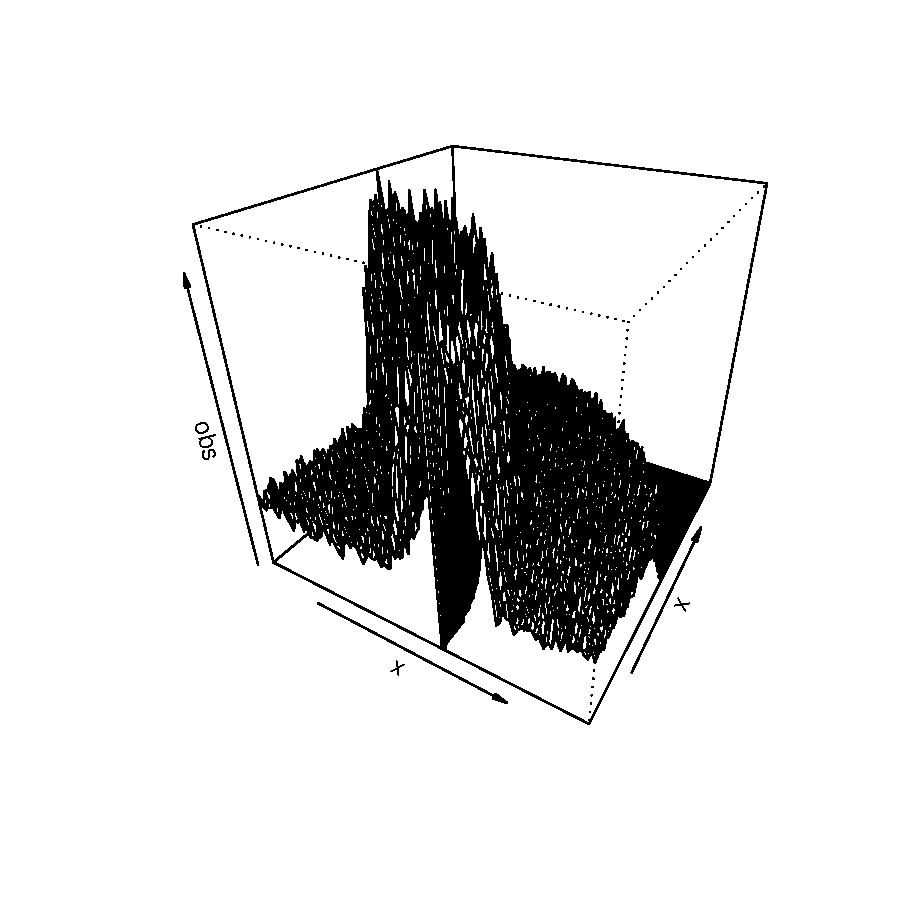
\includegraphics{RNG/images/nodeDensitySample.pdf}


Alternatively, we can draw the actual density
(as before) and then superimpose the scaled
counts:
{\footnotesize{
\begin{verbatim}
v = persp(x, x, outer(x, x, nodeDensity), phi = 30, theta = 30)
g = expand.grid(x, x)
oo = as.integer(obs)
points(trans3d(g[,1], g[,2], 4*oo/max(oo), v), col = "red", pch = "+")
\end{verbatim}
}}
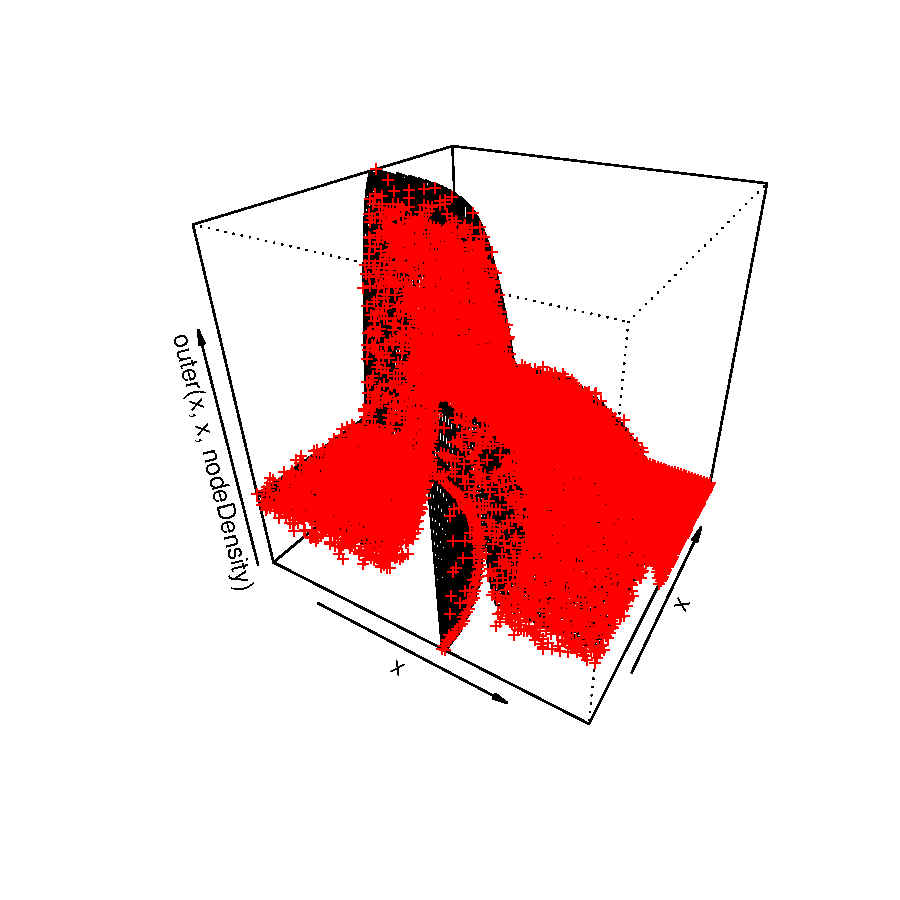
\includegraphics{RNG/images/nodeDensityPoints.pdf}
It is hard to see how good a fit this is.


We can compare the observed counts in each bin to the expected number
in each bin.  The expected number can be approximated by the average
$f(x, y)$ within the bin multiplied by the total number, i.e.
\Sexpression{nrow(p)}.
\begin{verbatim}
x = seq(.5, length = 100)
expected = outer(x, x, nodeDensity) * nrow(p)
\end{verbatim}
Of course, this approximation only works well when 
$f(x,y)$ is reasonably constant within a bin.
This is clearly not true for the high ridges.


We can also compute marginal and conditional distributions.  For $y =
0$, we should see the density being close to the front slice of the 2-D
density in the perspective plot:
\begin{verbatim}
curve(nodeDensity(x, rep(0, length(x))), 0, 100, n = 10000)
points(seq(.5, length = 100), 
   as.numeric(4*obs[,1]/max(obs[, 1])), col = "red")
\end{verbatim}
We can do this for arbitrary $y$
with the command
\begin{verbatim}
curve(nodeDensity(x, rep(y, length(x))), 0, 100, n = 10000)
points(seq(.5, length = 100), 
   as.numeric(4*obs[,as.integer(y)]/max(obs[, 1])), col = "red")
\end{verbatim}


Let's return to examining our function.  Note that we call
\SFunction{runif} for each pair $(x, y)$ and again for each $u$ to
determine if we accept the point.  The random number generation
functions in R can return $n$ values in a single call and this is much
more efficient than $n$ calls each returning a single observation.  We
can use this idea to make our function faster.  Firstly, we will try
to generate lots of values in a single step.  We will reject some, so
we will return and generate however many more are needed in the
subsequent attempts.  Each time, the number we need to generate should
be decreasing.  And in each iteration, we are generating numerous
values, not just a single value. So we are taking advantage of the
vectorized operations.

In addition to this speedup, we can also do a generic ``trick'' for
acceptance-rejection sampling.  Since we expect to reject some
proportion of the generated observations, we will generate more than
we need in the hope of getting the right number.  When asked for $n$
values, we generate $n' = k \times n$ values where $k > 1$.  By
carefully choosing $k$ (by theoretical or empirical reasoning), we can
find a trade-off between generating too many and not generating
enough.


A revised version of the function now looks like the following.
We create an empty answer object which is a matrix with 2 columns
and no rows! We will add our acceptable observations as we generate
them.
We increase the number we will generate by multiplying by
the user-specifiable \SArg{factor}.
In our case, for every observation we want, we will generate 3.

We then enter our acceptance-rejection loop,
continuing to sample until we have enough
observations.
For each iteration, we generate
\Svariable{nmore} candidate points.
Then we evaluate $f(x, y)$ at these points.
Then, we find out which are acceptable by generating
\Svariable{nmore} values from $U(0, c')$.
Note that we take advantage of the speed up here
of generating many values from this one distribution.
If we were not using a constant majorizing density, we
would not be able to do this. Instead, we would have
to generate each value from $U(0, c \times g(x, y))$.

Having determined the acceptable points, we append these to the answer
matrix. If the resulting matrix has $n$ or more rows, we can finish,
so we break from the loop.  Otherwise, we need to generate additional
observations and we need \Sexpression{n - row(ans)} of them.  So
again, we ask for \SArg{factor} times that many to take into account
the expected number of rejections.

At the end, we make certain to return only the first $n$ rows of the
answer matrix. If the caller asked for $n$, we must not give them back
$> n$ observations.

{\footnotesize{
\begin{verbatim}
rDensity =
function(n = 100, factor = 2.9, c.prime = 3.99)
{
   # Create an empty answer matrix with zero rows.
  ans = matrix(NA, 0, 2)

   # Determine how many we need to generate to get
   # the n that we want. 
  nmore = ceiling(factor*n)

   # This will store the proportion that were accepted each iteration.
  rate <- numeric(0)
  
  while(TRUE) {
     pos = matrix(runif(2*nmore, 0, 100), ncol = 2)
     f = nodeDensity(pos[,1], pos[,2])
     
     acc = (runif(nmore, 0, c.prime) < f)
     ans <- rbind(ans, pos[acc,])

     rate[as.character(nmore)] <- sum(acc)/nmore
     
     if(nrow(ans) >= n)
        break

     nmore =  ceiling(factor * (n - nrow(ans)))
   }

   # Limit the result to just the first n rows
   # in case we ended up with more accepted.
   ans = ans[1:n,]

   # Put the rate information on the object
   attr(ans, "rate") <- rate
   ans
}
\end{verbatim}
}}


Note that when we asked for $n$ values, we got back 
a matrix as expected, but there was also an attribute
named \SArg{rate} attached to it which we can access
as 
\begin{verbatim}
z = rDensity(100)
attr(z, "rate")
\end{verbatim}
This is a named vector.  Each element tells us what proportion of the
generate candidate points were accepted.  The name for that element
tells us how many candidate points there were.  This information tells
us the empirical probability of acceptance.  We can use this to
calibrate the function.  These are essentially estimates of $p$, the
probability of acceptance.  The variance of the estimate is $ \hat{p}
(1 - \hat{p})/n_i$, where $n_i$ is the number of items being sampled
of which $\hat{p}$ are rejected.  So we would want to take a weighted
average of these by using 1 over the variance as the weight.  And the
variance is essentially then 1 over the number of items that were up
for acceptance or rejection since $p$ is assumed to be the same.  So
the weights are 
\begin{verbatim}
w = as.integer(names(attr(z, "rate")))
w = w/sum(w)
\end{verbatim}
and our estimate is 
\begin{verbatim}
sum(attr(z, "rate")* w)
\end{verbatim}

At the end of each run of this function, we could update the default
value of the \SArg{factor} argument.  If our function had its own
environment, the updated estimate would be easy to store in the
environment.

Similarly, since we evaluate $f(x, y)$ many times, we can verify that
the values are all less than \SArg{c.prime}.  If we find one that
isn't, we can update the default value of \SArg{c.prime} to that newly
found maximum.  Again, if the function has its own environment, this
is easy to do.

The following code gives us what we want.
{\footnotesize{
\begin{verbatim}
rDensity =
function(n = 100, factor = 1/accRate, c.prime = maxDensity)
{
   # Create an empty answer matrix with zero rows.
  ans = matrix(NA, 0, 2)

   # Determine how many we need to generate to get
   # the n that we want. 
  nmore = ceiling(factor*n)

   # This will store 
  rate <- numeric(0)
  
  while(TRUE) {
     pos = matrix(runif(2*nmore, 0, 100), ncol = 2)
     f = nodeDensity(pos[,1], pos[,2])
     
     m = max(f)
     if(m > c.prime) { 
       warning("new maximum value for density found in rDensity. 
         Check previous output!")
       maxDensity <<- m
     }

     acc = (runif(nmore, 0, c.prime) < f)
     ans <- rbind(ans, pos[acc,])

     rate[as.character(nmore)] <- sum(acc)/nmore
     
     if(nrow(ans) >= n)
        break

     nmore =  ceiling(factor * (n - nrow(ans)))
   }

   # Limit the result to just the first n rows
   # in case we ended up with more accepted.
   ans = ans[1:n,]

   # Put the rate information on the object
   attr(ans, "rate") <- rate

    # Now update the acceptance rate estimate.
   rate <- structure(c(accRate, rate), names = c(names(accRate), names(rate)))
   n =  sum(as.integer(names(rate)))
   w = as.integer(names(rate))/ n
   accRate <<- sum(w * rate)
   names(accRate) <<- as.character(n)
  browser()

   ans
}
environment(rDensity) <- new.env()
environment(rDensity)$maxDensity <- 3.99
environment(rDensity)$accRate <- c("1000" = 1/2.9)
\end{verbatim}
}}

So this version is self-correcting and converges to the appropriate factor.
(Check the details.)
